%=============================================================================
% Thesis Template in LaTex
%
% File:  04-06-Szenarien.tex -- Fallstudie/Modellierung der ungewissen Parameter
% Author(s): Jürgen Hackl <hackl@ibi.baug.ethz.ch>
%            Clemens Kielhauser <kielhauser@ibi.baug.ethz.ch>
%
% Creation:  27 Jan 2014
% Time-stamp: <Tue 2013-08-13 20:14 juergen>
%
% Copyright (c) 2014 Infrastructure Management Group (IMG)
%               http://ibi.ethz.ch
%
% More information on LaTeX: http://www.latex-project.org/
%=============================================================================

% Unterkapitel Szenarien
% ---------

\subsubsection*{Bevölkerungswachstum}
\label{subsubsec:Bevölkerung}

Wie in Kapitel \ref{chap:Fallstudie} erwähnt, ist das DTV mehrheitlich von der zukünftigen demographischen Entwicklung abhängig.
Um den Effekt, den das Bevölkerungswachstum auf das DTV haben wird, modellieren zu können, orientiere ich mich an den Wachstumsprognosen der Stadt Uster.
Die zu erwartende Bevölkerungsentwicklung habe ich dem Kapitel 3 \textit{Stadt Uster im Porträt} des STEK entnommen und wird nachfolgend kurz beschrieben. 

\begin{description}
\item[Stagnation] \hfill \\
Geschätzte Anzahl an Einwohner im Jahr 2035: 38'760 \\
$\Rightarrow$ + 188 Einwohner/Jahr \\ $\Rightarrow$ + 0.5\% pro Jahr gegenüber 2015
\item[Trend restriktiv] \hfill \\
Geschätzte Anzahl an Einwohner im Jahr 2035: 42'260 \\ 
$\Rightarrow$ + 363 Einwohner/Jahr \\ $\Rightarrow$ + 1\% pro Jahr gegenüber 2015
\item[Trend Prosperität] \hfill \\
Geschätzte Anzahl an Einwohner im Jahr 2035: 45'620 \\ 
$\Rightarrow$+ 531 Einwohner/Jahr \\ $\Rightarrow$ + 1.5\% pro Jahr gegenüber 2015
\end{description}

Anhand dieser Wachstumsprognosen und unter der Annahme eines linearen Wachstums, definiere ich die drei nachfolgend dargestellten Szenarien. Mit diesen Szenarien werde ich in einem nächsten Schritt den zukünftigen DTV für den MIV und den Langsamverkehr, sprich Veloverkehr, am Bahnübergang Brunnenstrasse ermitteln.
Ausgehend vom DTV des MIV im Jahr 2016 und den Wachstumsraten der Szenarien habe ich die jährliche Zunahme an Motorfahrzeugen ermittelt. Im Jahr 2016 lag das DTV des MIV am Bahnübergang bei 12'023 Motorfahrzeugen pro Tag. \\ (\cite{GIS})

\begin{itemize}
\item Szenario: SB 1
	\begin{itemize}
	\item Grundlage: Stagnation $\Rightarrow$ jährliches Wachstum um 0.5\%
	\item Jährliche Zunahme DTV: 60 Fahrzeuge
	\item Eintrittswahrscheinlichkeit: 25\%
	\end{itemize}
\item Szenario: SB 2
	\begin{itemize}
	\item Grundlage: Trend restriktiv  $\Rightarrow$ jährliches Wachstum um 1 \%
	\item Jährliche Zunahme DTV: 120 Fahrzeuge
	\item Eintrittswahrscheinlichkeit: 50\%
	\end{itemize}
\item Szenario: SB 3
	\begin{itemize}
	\item Grundlage: Trend Prosperität  $\Rightarrow$ jährliches Wachstum um 1.5\%
	\item Jährliche Zunahme DTV: 180 Fahrzeuge
	\item Eintrittswahrscheinlichkeit: 25\%
	\end{itemize}
\end{itemize}


Die Wahrscheinlichkeit das Szenario SB 2 eintritt und das DTV jährlich um 120 Fahrzeuge zunimmt, bewerte ich mit 50\%. Dies erfolgt unter der Annahme, dass der restriktive Trend das minimale Wachstumsziel von 20\% wiederspiegelt, welches gemäss dem STEK mit grösster Wahrscheinlichkeit eintreten wird, und da dieses Szenario den kantonalen Prognosen entspricht, erachte ich dieses Szenario als das wahrscheinlichste und bewerte es dementsprechend.

Das es zu einem verstärktem Wachstum von 1.5\% und somit zu einer jährlichen Zunahme von 180 Fahrzeugen am DTV kommt, erachte ich nach den Angaben des STEK als unwahrscheinlich, da ein übermässiges Bevölkerungswachstum aufgrund der nur beschränkt vorhandenen Kapazitäten zur Erweiterung der Wohnangebots, nur bedingt möglich ist. 

Das es zu einer Stagnation des Bevölkerungswachstums und im Zuge dieser Modellierung zu einem Verkehrswachstum von 0.5\% und einer jährlichen Zunahme von 60 Fahrzeugen am DTV kommt, erachte ich in Anbetracht der Prognosen zur demographische Entwicklung im Kanton Zürich, als unwahrscheinlich. Deshalb bewerte ich die Szenarien SB 1 und SB 3 mit jeweils 25\%.

Mithilfe der verschiedenen Wachstumsraten $WR_{s}$ der Szenarien und der Formel \ref{eq.11} berechne ich das $DTV_{i}$ im Jahr $t_{i}$. \\
Der DTV des Jahres 2016 lag, wie oben erwähnt, bei 12'023 Motorfahrzeuge pro Tag. Diesen Wert nutze ich als Start- sowie Basiswert meiner Berechnungen. 

\begin{equation}
DTV_{i} = DTV_{2016} + \bigl( t_{i} - t_{2016} \bigr) \cdot \bigl[WR_{s}\bigr] \cdot DTV_{2016}
\label{eq.11}
\end{equation}

Da die Anzahl Velos, die den Bahnübergang Brunnenstrasse täglich passieren, nicht von einer Verkehrsmessstelle gezählt werden, muss diese Information aus dem MIV hergeleitet werden. Dies erfolgt mithilfe der Daten der Verkehrsmessstelle an der etwas südlich von Uster gelegenen Seefeldstrasse, welche Niederuster mit Riedikon verbindet. 
Der im Jahr 2019 gemessen durchschnittliche DTV lag bei 8818 Motorfahrzeugen für das MIV und 913 Velos. Daraus ergibt sich einen Veloanteil von 10.35\%. \footcite{MIVSeefeld}\footcite{VeloSeefeld}

\begin{align*}
\mu &= \frac{DTV_{Velo,Seefeldstrasse}}{DTV_{MIV,Seefeldstrasse}}   \\[2ex]
DTV_{Velo} &= DTV_{MIV} \cdot \mu_{Velo} 
\end{align*}

In den Abbildung \ref{fig:DTV} sind die Ergebnisse meiner Modellierung des DTV am Bahnübergang Brunnenstrasse dargestellt, die ich für die Berechnung der Kosten der Varianten verwenden werde. Eine ausführliche Tabelle aller modellierten DTV-Werte findet sich unter Abschnitt \ref{subsec:DTVModellierung}

\begin{figure}[h!]
  \centering
  \subfloat[][]{\label{fig:04-06-02-DTV(MIV)}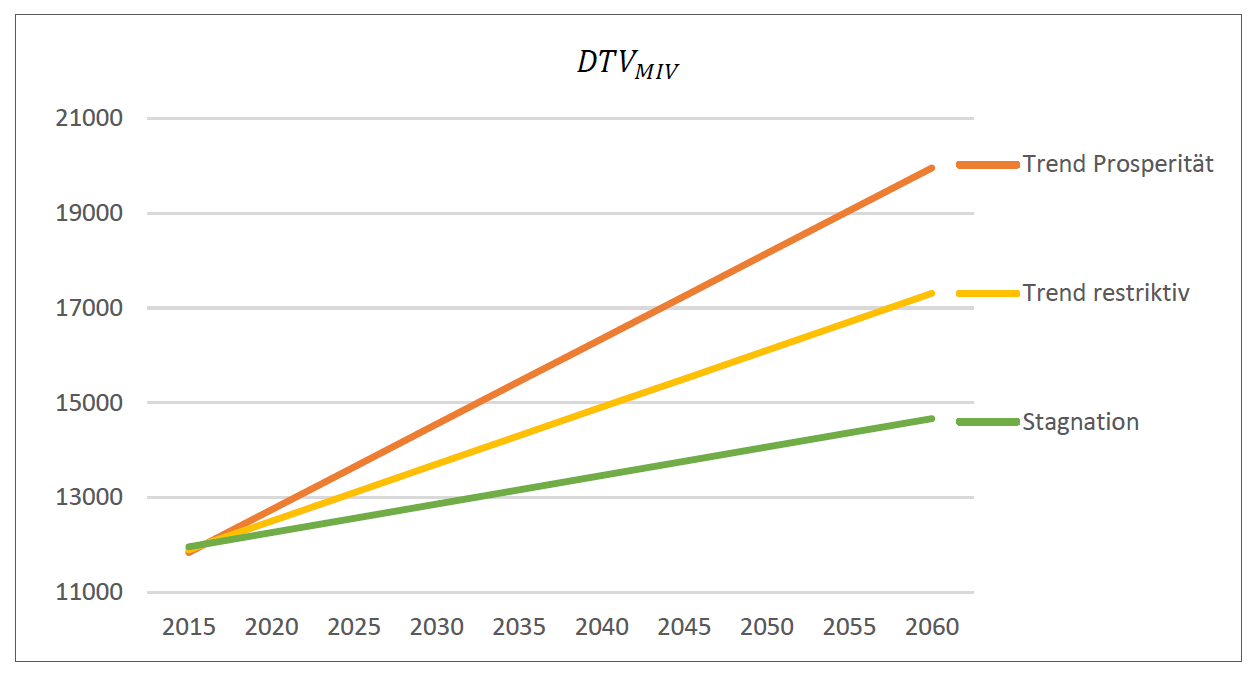
\includegraphics[width=.5\textwidth]{./figures/f-04-06-02-DTV(MIV)-SzenarienBev-Wachstum}}
  \hfill
  \subfloat[][]{\label{fig:04-06-03-DTV(VELO)}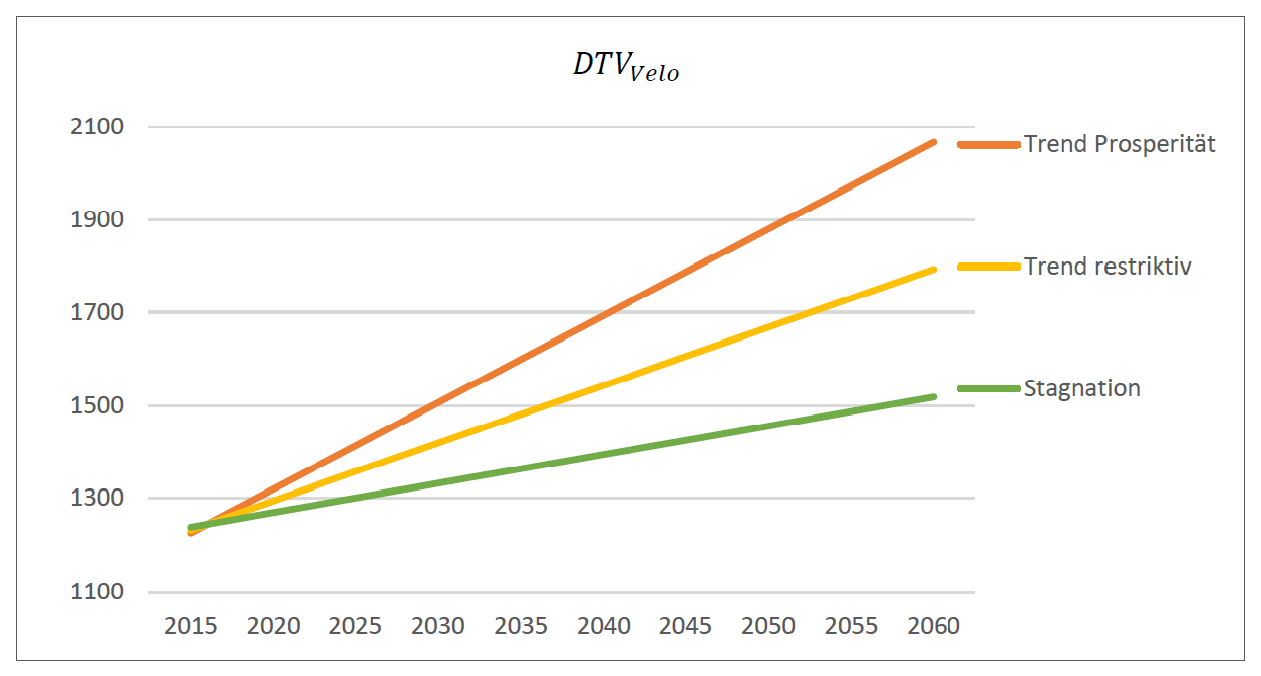
\includegraphics[width=.5\textwidth]{./figures/f-04-06-03-DTV(VELO)-SzenarienBev-wachstum}}
\caption[DTV Brunnenstrasse]{DTV an der Brunnenstrasse}
  \label{fig:DTV}
\end{figure}



\subsubsection*{Umsetzung STEK}
\label{subsubsec:Umsetzung}

Die folgenden Szenarien modellieren die Effekte, den die in Abschnitt \ref{subsec:Modellierung} unter dem Stickwort \textit{Umsetzung STEK} zusammengefassten Einflussfaktoren, auf den $DTV_{Velo}$ haben werden. 

Das meines Erachtens mit grösster Wahrscheinlichkeit eintretende Szenario entspricht der Verkehrsprognose des Bundes, die eine Zunahme der Verkehrsleistung des Langsamverkehrs bis 2040 gegenüber 2010, um 32\% erwartet. (\cite{Perspektive2040}) 

Um die Ober- sowie Untergrenze meiner Prognose ermitteln zu können, orientiere ich mich ein weiteres Mal am STEK. Mithilfe der unter Kapitel 10 \textit{Stadt Uster im Porträt} des STEK vorgestellten Wachstumsprognosen für die Bevölkerungsentwicklung sowie der in Kapitel 7 \textit{Mobilität} des STEK gemäss regionalem Richtplan erstellten Verkehrsprognose für den Anteil der Velofahrer am Gesamtverkehr, erstelle ich zwei weitere Szenarien. 
Einerseits berücksichtige ich den Fall einer ungenügenden Umsetzung der Leitziele und der daraus resultierenden stagnierenden Entwicklung des Veloverkehrs. Andererseits den Fall einer maximalen Umsetzung aller Ziele in Verbindung mit einer Verschiebung des Innerstädtischen Modalsplit in Richtung Langsamverkehr.

\pagebreak

\begin{description}
\item[Stagnation] \hfill \\
Prognose gemäss STEK: $\Rightarrow$ jährliches Wachstum: 0.54 \% 
\item[Verkehrsperspektiven 2040] \hfill \\
Prognostizierte Zunahme der Verkehrsleistung: 32\% $\Rightarrow$ jährliches Wachstum: 1.3 
\item[Umsetzung maximal] \hfill \\
Prognose gemäss STEK und regionalem Richtplan: $\Rightarrow$ jährliches Wachstum: 2 \% 
\end{description}

Eine Stagnation erachte ich unter Berücksichtigung der Entwicklung des Langsamverkehrs über die letzten zehn Jahre, als unwahrscheinlich und bewerte das Eintreten dieser Prognose demzufolge mit 5\%. \\
Dass es zu einem Wachstum gemäss der Prognose des Bundes kommen wird, erachte ich nach der Konsultation weitere Verkehrsprognosen, als das Szenario, welches mit grösster Wahrscheinlichkeit eintreten wird. Daher bewerte ich dieses Szenario mit einer Eintrittswahrscheinlichkeit von 57.5\%. \\
Dass alle Ziele maximal erfüllt werden und eine Verschiebung des innerstädtischen Modal-Split stattfindet, erachte ich mit 32.5\% als deutlich plausibler als die Stagnation, jedoch als unwahrscheinlicher als die Prognose des Bundes. 

\begin{itemize}
\item Szenario: SU 1
	\begin{itemize}
	\item Grundlage: Stagnation 
	\item Eintrittswahrscheinlichkeit: 5\%
	\end{itemize}
\item Szenario: SB 2
	\begin{itemize}
	\item Grundlage: Verkehrsperspektiven 2040
	\item Eintrittswahrscheinlichkeit: 57.5\%
	\end{itemize}
\item Szenario: SB 3
	\begin{itemize}
	\item Grundlage: Umsetzung maximal
	\item Eintrittswahrscheinlichkeit: 32.5\%
	\end{itemize}
\end{itemize}

Anhand der zu Beginn dieses Abschnitts definierten Wachstumsraten, sowie ausgehend von den Messwerten des täglichen Veloverkehrs im Jahr 2016, habe ich die Anzahl Velos, die in jedem Szenario zusätzlich pro Tag auf der Infrastruktur unterwegs sein werden, ermittelt. 
Die Anzahl Velos die im Jahr 2016 täglich den Bahnübergang nutzten, lag, gemäss Abschnitt \ref{subsubsec:Bevölkerung}, bei 1245.

Das Szenario SU 1 führt somit zu einer Erhöhung des täglichen Veloverkehrs um 7 Velos pro Jahr, das Szenario SU 2 zu einer Zunahme von 16 Velos pro Jahr und das Szenario SB 3 zu einer Erhöhung des $DTV_{Velo}$ um 25 Velos pro Jahr. 
Mit diesen Angaben berechne ich die Anzahl Velos, die je nach Szenario, zusätzlich zu den in Abschnitt \ref{subsubsec:Bevölkerung} berechneten DTV-Werten, auf der Infrastruktur unterwegs sein werden.

\pagebreak

% ===========================================================================
% EOF
%

%%% Local Variables:
%%% mode: latex
%%% TeX-master: "../main"
%%% End:
